\documentclass[12pt,a4paper]{article}
\usepackage[utf8]{inputenc}
\usepackage[T1]{fontenc}
\usepackage{amsmath}
\usepackage{geometry}
\usepackage{setspace}
\usepackage{parskip}
\usepackage{enumitem}
\usepackage{booktabs}
\usepackage{longtable}
\usepackage{array}
\usepackage{xcolor}
\usepackage{hyperref}
\usepackage{float}
\usepackage{tikz}
\usetikzlibrary{arrows.meta,positioning,calc,matrix,fit,backgrounds}
\usepackage{fancyhdr}
\usepackage{titlesec}

\geometry{left=2.5cm,right=2.5cm,top=2.5cm,bottom=2.5cm,headheight=14.5pt}
\onehalfspacing
\hypersetup{colorlinks=true,linkcolor=black,urlcolor=blue,pdftitle={Diagramas C4 - Sistema Integral de Gestión de Eventos},pdfauthor={Samuel Contreras}}

\definecolor{azul}{RGB}{31,78,121}
\definecolor{gris}{RGB}{242,242,242}
\definecolor{grisoscuro}{RGB}{80,80,80}
\definecolor{verde}{RGB}{39,120,70}
\definecolor{naranja}{RGB}{230,126,34}
\definecolor{morado}{RGB}{106,27,154}

\titleformat{\section}{\Large\bfseries\color{azul}}{\thesection.}{0.5em}{}
\titleformat{\subsection}{\large\bfseries}{\thesubsection.}{0.5em}{}
% Etiquetas en español (sin babel, que no está disponible en este entorno)
\renewcommand{\contentsname}{Índice}
\renewcommand{\figurename}{Figura}
\renewcommand{\tablename}{Tabla}

\pagestyle{fancy}
\fancyhf{}
\fancyhead[L]{Sistema Integral de Gestión de Eventos}
\fancyhead[R]{Diagramas C4}
\fancyfoot[C]{\thepage}

\begin{document}

\begin{titlepage}
\centering
\vspace*{2cm}
{\Huge\bfseries Sistema Integral de Gestión de Eventos\par}
\vspace{0.7cm}
{\Large Arquitectura de Software\par}
\vspace{1.2cm}
{\Large\bfseries Diagramas de Arquitectura --- Modelo C4\par}
\vspace{2cm}
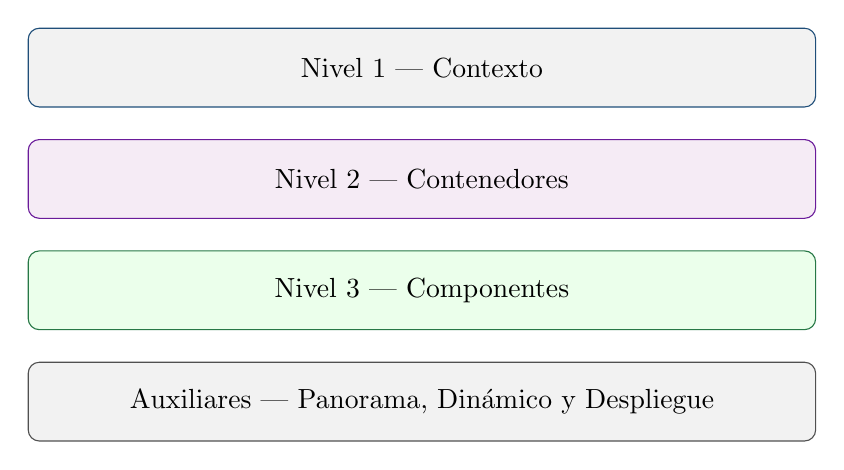
\begin{tikzpicture}
\node[draw=azul,rounded corners,fill=gris,minimum width=10cm,minimum height=1cm,align=center]
{Nivel 1 --- Contexto};
\node[draw=morado,rounded corners,fill=violet!8,minimum width=10cm,minimum height=1cm,below=0.4cm of current bounding box.south,align=center]
{Nivel 2 --- Contenedores};
\node[draw=verde,rounded corners,fill=green!8,minimum width=10cm,minimum height=1cm,below=0.4cm of current bounding box.south,align=center]
{Nivel 3 --- Componentes};
\node[draw=grisoscuro,rounded corners,fill=gris,minimum width=10cm,minimum height=1cm,below=0.4cm of current bounding box.south,align=center]
{Auxiliares --- Panorama, Dinámico y Despliegue};
\end{tikzpicture}
\vfill
\begin{tabular}{rl}
\textbf{Materia:} & Arquitectura de Software\\
\textbf{Estudiante:} & Samuel Contreras\\
\textbf{Fecha:} & Agosto de 2026\\
\textbf{Documento base:} & Atributos de Calidad y Propuesta Arquitectónica
\end{tabular}
\end{titlepage}

\tableofcontents
\newpage

\section{Introducción}

Este documento complementa a \textbf{Atributos de Calidad y Propuesta Arquitectónica} y presenta,
de forma independiente, los diagramas de arquitectura del \textbf{Sistema Integral de Gestión de
Eventos} siguiendo el \textbf{modelo C4} (Simon Brown). Incluye los tres diagramas jerárquicos
principales --- \textbf{Contexto} (Nivel 1), \textbf{Contenedores} (Nivel 2) y \textbf{Componentes}
(Nivel 3) --- y los tres diagramas auxiliares del modelo: \textbf{Panorama de Sistemas} (\textit{System
Landscape}), \textbf{Dinámico} (\textit{Dynamic}) y \textbf{Despliegue} (\textit{Deployment}). No se
incluye el Nivel 4 (Código) porque la guía oficial del modelo solo lo recomienda para componentes
especialmente críticos, y normalmente se genera de forma automática con herramientas de IDE a
partir del código fuente ya escrito --- que todavía no existe para este proyecto.

Cada diagrama incluye título, tipo, alcance, leyenda de notación y una tabla de relaciones con la
tecnología asociada a cada una, en cumplimiento del checklist oficial de
\href{https://c4model.com/diagrams/checklist}{c4model.com/diagrams/checklist}, verificado al
final de este documento.

\section{Nivel 1 — Diagrama de contexto}

\textbf{Tipo:} diagrama de contexto del sistema. \textbf{Alcance:} muestra el Sistema Integral de
Gestión de Eventos como caja negra, los roles de usuario que interactúan con él y los sistemas
externos de los que depende. \textbf{Audiencia:} técnica y no técnica.

\begin{figure}[H]
\centering
\resizebox{\textwidth}{!}{
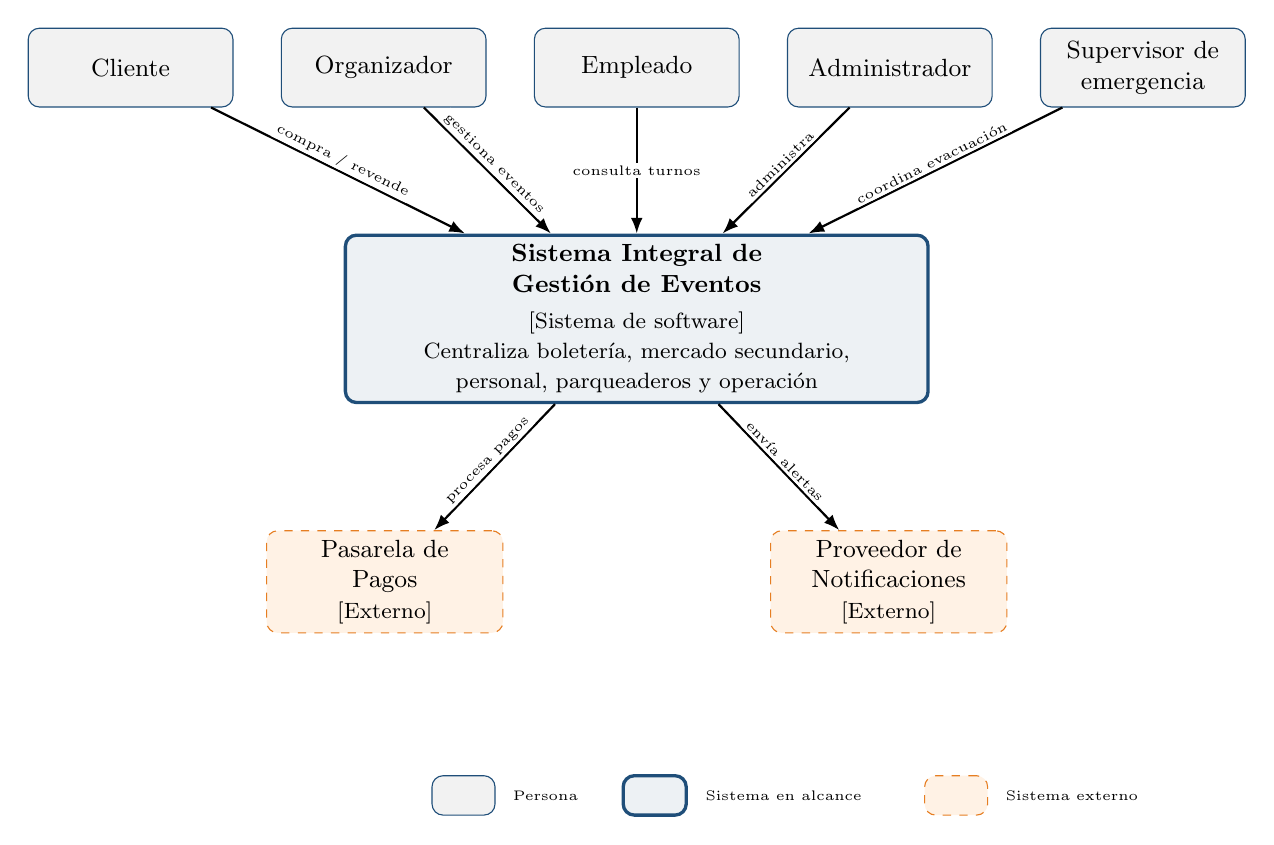
\begin{tikzpicture}[
persona/.style={draw=azul,rounded corners,fill=gris,minimum width=2.6cm,minimum height=1cm,align=center,font=\small},
sistemabox/.style={draw=azul,very thick,rounded corners,fill=azul!8,minimum width=7.4cm,minimum height=2.1cm,align=center,font=\small},
ext/.style={draw=naranja,rounded corners,dashed,fill=orange!10,minimum width=3cm,minimum height=1cm,align=center,font=\small},
arr/.style={-{Latex[length=2mm]},thick},
lbl/.style={font=\tiny,fill=white,inner sep=1pt}
]
\node[persona] (cliente) {Cliente};
\node[persona,right=6mm of cliente] (organizador) {Organizador};
\node[persona,right=6mm of organizador] (empleado) {Empleado};
\node[persona,right=6mm of empleado] (admin) {Administrador};
\node[persona,right=6mm of admin] (supervisor) {Supervisor de\\emergencia};

\node[sistemabox,below=16mm of empleado] (sistema)
  {\textbf{Sistema Integral de}\\\textbf{Gestión de Eventos}\\[2pt]
  \footnotesize [Sistema de software]\\
  \footnotesize Centraliza boletería, mercado secundario,\\
  \footnotesize personal, parqueaderos y operación};

\node[ext,below=16mm of sistema,xshift=-32mm] (pagos) {Pasarela de\\Pagos\\\footnotesize [Externo]};
\node[ext,below=16mm of sistema,xshift=32mm] (notif) {Proveedor de\\Notificaciones\\\footnotesize [Externo]};

\draw[arr] (cliente) -- (sistema) node[lbl,midway,sloped,above] {compra / revende};
\draw[arr] (organizador) -- (sistema) node[lbl,midway,sloped,above] {gestiona eventos};
\draw[arr] (empleado) -- (sistema) node[lbl,midway] {consulta turnos};
\draw[arr] (admin) -- (sistema) node[lbl,midway,sloped,above] {administra};
\draw[arr] (supervisor) -- (sistema) node[lbl,midway,sloped,above] {coordina evacuación};
\draw[arr] (sistema) -- (pagos) node[lbl,midway,sloped,above] {procesa pagos};
\draw[arr] (sistema) -- (notif) node[lbl,midway,sloped,above] {envía alertas};

\node[persona,minimum width=8mm,minimum height=5mm,font=\tiny,below=18mm of pagos,xshift=10mm] (leg1) {};
\node[font=\tiny,right=1mm of leg1] {Persona};
\node[sistemabox,minimum width=8mm,minimum height=5mm,font=\tiny,right=16mm of leg1] (leg2) {};
\node[font=\tiny,right=1mm of leg2] {Sistema en alcance};
\node[ext,minimum width=8mm,minimum height=5mm,font=\tiny,right=30mm of leg2] (leg3) {};
\node[font=\tiny,right=1mm of leg3] {Sistema externo};
\end{tikzpicture}
}
\caption{Diagrama de contexto (Nivel 1, modelo C4).}
\end{figure}

\begin{longtable}{p{3cm}p{3cm}p{6.5cm}p{2.3cm}}
\toprule
\textbf{Origen} & \textbf{Destino} & \textbf{Descripción} & \textbf{Tecnología}\\
\midrule
Cliente & Sistema & Consulta eventos, compra y revende entradas, reserva parqueadero. & HTTPS\\
Organizador & Sistema & Crea eventos, asigna personal y coordina la operación. & HTTPS\\
Empleado & Sistema & Consulta turnos y registra ingreso/salida. & HTTPS\\
Administrador & Sistema & Administra usuarios, personal y configuración. & HTTPS\\
Supervisor de emergencia & Sistema & Activa y coordina el protocolo de evacuación. & HTTPS\\
Sistema & Pasarela de Pagos & Procesa compras, reventas y reembolsos. & HTTPS/REST\\
Sistema & Proveedor de Notificaciones & Envía notificaciones push, correo y SMS. & HTTPS/REST\\
\bottomrule
\caption{Relaciones del diagrama de contexto.}
\end{longtable}

\section{Nivel 2 — Diagrama de contenedores}

\textbf{Tipo:} diagrama de contenedores. \textbf{Alcance:} zoom dentro del sistema, mostrando las
aplicaciones desplegables, los microservicios de dominio y la infraestructura de soporte.
\textbf{Audiencia:} arquitectos y desarrolladores.

\begin{figure}[H]
\centering
\resizebox{\textwidth}{!}{
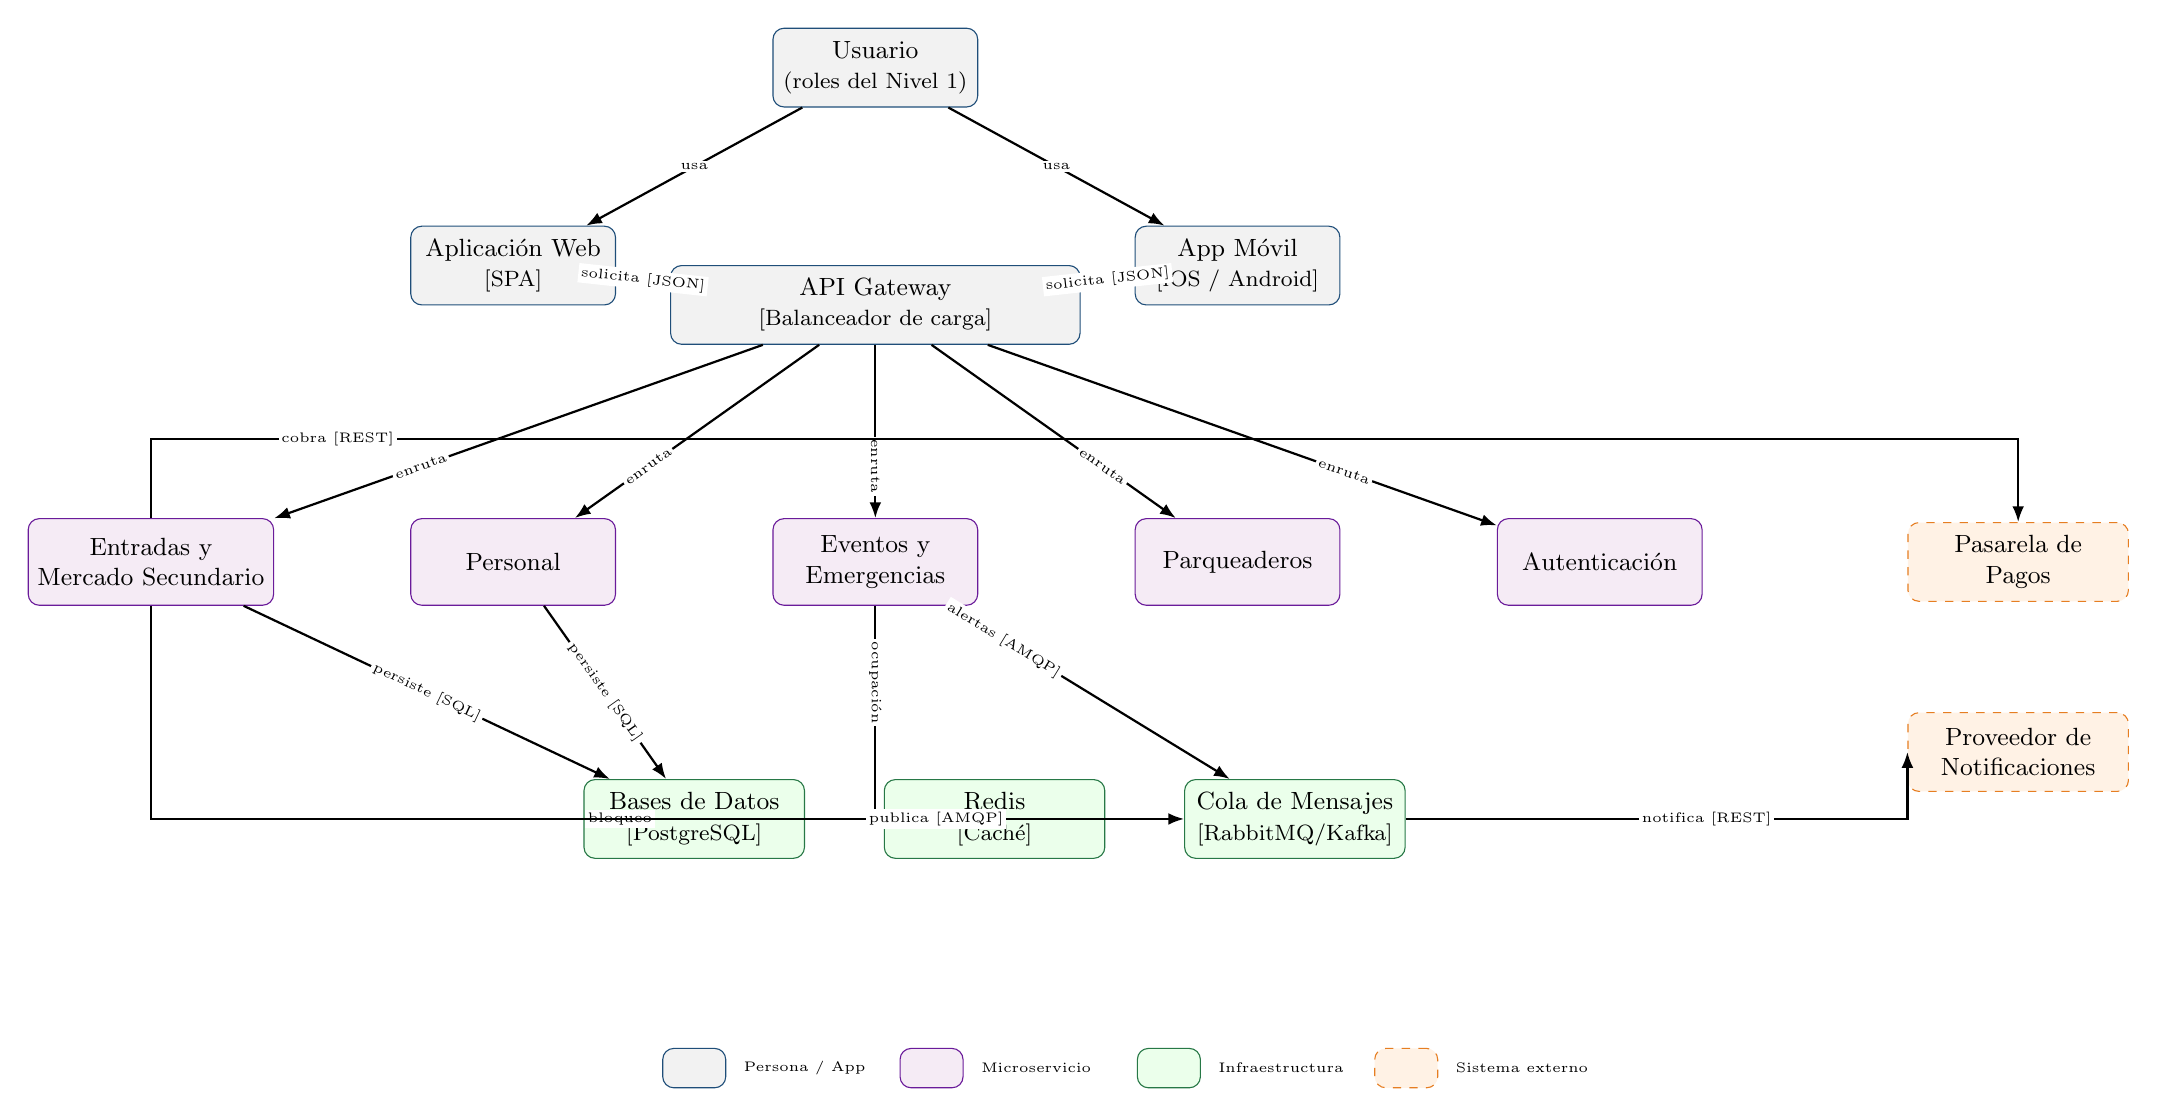
\begin{tikzpicture}[
persona/.style={draw=azul,rounded corners,fill=gris,minimum width=2.6cm,minimum height=1cm,align=center,font=\small},
contenedor/.style={draw=azul,rounded corners,fill=gris,minimum width=2.6cm,minimum height=1cm,align=center,font=\small},
microservicio/.style={draw=morado,rounded corners,fill=violet!8,minimum width=2.6cm,minimum height=1.1cm,align=center,font=\small},
infra/.style={draw=verde,rounded corners,fill=green!8,minimum width=2.8cm,minimum height=1cm,align=center,font=\small},
ext/.style={draw=naranja,rounded corners,dashed,fill=orange!10,minimum width=2.8cm,minimum height=1cm,align=center,font=\small},
arr/.style={-{Latex[length=2mm]},thick},
lbl/.style={font=\tiny,fill=white,inner sep=1pt}
]
\node[persona] (usuario) {Usuario\\\footnotesize (roles del Nivel 1)};

\node[contenedor,below=15mm of usuario,xshift=-46mm] (web) {Aplicación Web\\\footnotesize [SPA]};
\node[contenedor,below=15mm of usuario,xshift=46mm] (movil) {App Móvil\\\footnotesize [iOS / Android]};

\node[contenedor,below=20mm of usuario,minimum width=5.2cm] (gw) {API Gateway\\\footnotesize [Balanceador de carga]};

\node[microservicio,below=22mm of gw,xshift=-92mm] (ms1) {Entradas y\\Mercado Secundario};
\node[microservicio,below=22mm of gw,xshift=-46mm] (ms2) {Personal};
\node[microservicio,below=22mm of gw] (ms3) {Eventos y\\Emergencias};
\node[microservicio,below=22mm of gw,xshift=46mm] (ms4) {Parqueaderos};
\node[microservicio,below=22mm of gw,xshift=92mm] (ms5) {Autenticación};

\node[infra,below=22mm of ms2,xshift=23mm] (bd) {Bases de Datos\\\footnotesize [PostgreSQL]};
\node[infra,right=10mm of bd] (redis) {Redis\\\footnotesize [Caché]};
\node[infra,right=10mm of redis] (cola) {Cola de Mensajes\\\footnotesize [RabbitMQ/Kafka]};

\node[ext,right=26mm of ms5] (pagos2) {Pasarela de\\Pagos};
\node[ext,below=14mm of pagos2] (notif2) {Proveedor de\\Notificaciones};

\draw[arr] (usuario) -- (web) node[lbl,midway] {usa};
\draw[arr] (usuario) -- (movil) node[lbl,midway] {usa};
\draw[arr] (web) -- (gw) node[lbl,midway,sloped] {solicita [JSON]};
\draw[arr] (movil) -- (gw) node[lbl,midway,sloped] {solicita [JSON]};
\foreach \m in {ms1,ms2,ms3,ms4,ms5} \draw[arr] (gw) -- (\m) node[lbl,pos=0.7,sloped] {enruta};

\draw[arr] (ms1) -- (bd) node[lbl,midway,sloped] {persiste [SQL]};
\draw[arr] (ms2) -- (bd) node[lbl,midway,sloped] {persiste [SQL]};
\draw[arr] (ms1) |- (redis) node[lbl,pos=0.82] {bloqueo};
\draw[arr] (ms3) |- (redis) node[lbl,pos=0.18,sloped] {ocupación};
\draw[arr] (ms1) |- (cola) node[lbl,pos=0.88] {publica [AMQP]};
\draw[arr] (ms3) -- (cola) node[lbl,pos=0.2,sloped] {alertas [AMQP]};
\draw[arr] (ms1.north) |- ($(ms1.north)+(0,10mm)$) -| (pagos2.north) node[lbl,pos=0.05,sloped] {cobra [REST]};
\draw[arr] (cola.east) -| (notif2.west) node[lbl,pos=0.3] {notifica [REST]};

\node[persona,minimum width=8mm,minimum height=5mm,font=\tiny,below=24mm of bd] (leg1) {};
\node[font=\tiny,right=1mm of leg1] {Persona / App};
\node[microservicio,minimum width=8mm,minimum height=5mm,font=\tiny,right=22mm of leg1] (leg2) {};
\node[font=\tiny,right=1mm of leg2] {Microservicio};
\node[infra,minimum width=8mm,minimum height=5mm,font=\tiny,right=22mm of leg2] (leg3) {};
\node[font=\tiny,right=1mm of leg3] {Infraestructura};
\node[ext,minimum width=8mm,minimum height=5mm,font=\tiny,right=22mm of leg3] (leg4) {};
\node[font=\tiny,right=1mm of leg4] {Sistema externo};
\end{tikzpicture}
}
\caption{Diagrama de contenedores (Nivel 2, modelo C4).}
\end{figure}

\begin{longtable}{p{3.2cm}p{3.2cm}p{5.7cm}p{2.3cm}}
\toprule
\textbf{Origen} & \textbf{Destino} & \textbf{Descripción} & \textbf{Tecnología}\\
\midrule
App Web / Móvil & API Gateway & Envía las solicitudes del usuario al backend. & HTTPS/JSON\\
API Gateway & Microservicios & Enruta cada solicitud al servicio correspondiente y balancea la carga. & HTTPS/JSON\\
Servicio de Entradas & Bases de Datos & Persiste entradas, publicaciones y transferencias. & SQL\\
Servicio de Entradas & Redis & Bloquea temporalmente una publicación durante el checkout. & Redis\\
Eventos/Emergencias & Redis & Actualiza el estado de ocupación de zonas en tiempo real. & Redis\\
Servicio de Entradas & Cola de Mensajes & Publica el evento de transferencia completada. & AMQP\\
Eventos/Emergencias & Cola de Mensajes & Publica alertas de evacuación. & AMQP\\
Servicio de Entradas & Pasarela de Pagos & Procesa el cobro de una compra o reventa. & HTTPS/REST\\
Cola de Mensajes & Proveedor de Notificaciones & Dispara notificaciones push, correo y SMS. & HTTPS/REST\\
\bottomrule
\caption{Relaciones del diagrama de contenedores.}
\end{longtable}

\section{Nivel 3 — Diagrama de componentes}

\textbf{Tipo:} diagrama de componentes. \textbf{Alcance:} zoom dentro del contenedor
\textit{Servicio de Entradas y Mercado Secundario} (caso de uso complejo CU-006), mostrando sus
componentes internos y su relación con los contenedores de los niveles anteriores.
\textbf{Audiencia:} arquitectos y desarrolladores.

\begin{figure}[H]
\centering
\resizebox{\textwidth}{!}{
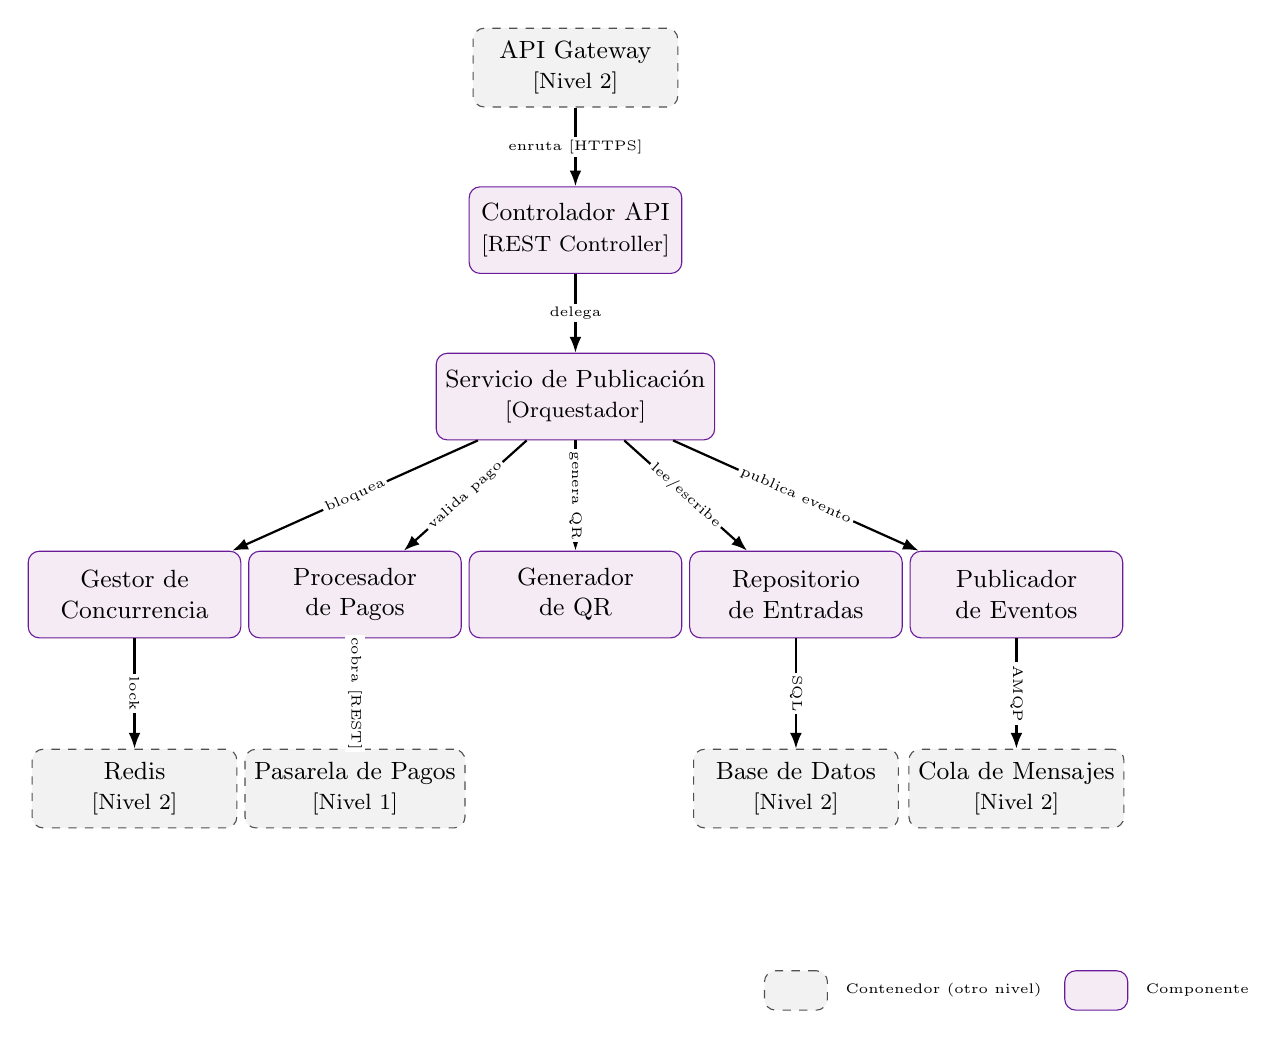
\begin{tikzpicture}[
referencia/.style={draw=grisoscuro,rounded corners,dashed,fill=gris,minimum width=2.6cm,minimum height=1cm,align=center,font=\small},
componente/.style={draw=morado,rounded corners,fill=violet!8,minimum width=2.7cm,minimum height=1.1cm,align=center,font=\small},
arr/.style={-{Latex[length=2mm]},thick},
lbl/.style={font=\tiny,fill=white,inner sep=1pt}
]
\node[referencia] (gw) {API Gateway\\\footnotesize [Nivel 2]};
\node[componente,below=10mm of gw] (ctrl) {Controlador API\\\footnotesize [REST Controller]};
\node[componente,below=10mm of ctrl] (pub) {Servicio de Publicación\\\footnotesize [Orquestador]};

\node[componente,below=14mm of pub,xshift=-56mm] (conc) {Gestor de\\Concurrencia};
\node[componente,below=14mm of pub,xshift=-28mm] (pago) {Procesador\\de Pagos};
\node[componente,below=14mm of pub] (qr) {Generador\\de QR};
\node[componente,below=14mm of pub,xshift=28mm] (repo) {Repositorio\\de Entradas};
\node[componente,below=14mm of pub,xshift=56mm] (evt) {Publicador\\de Eventos};

\node[referencia,below=14mm of conc] (redis) {Redis\\\footnotesize [Nivel 2]};
\node[referencia,below=14mm of pago] (pasarela) {Pasarela de Pagos\\\footnotesize [Nivel 1]};
\node[referencia,below=14mm of repo] (bd) {Base de Datos\\\footnotesize [Nivel 2]};
\node[referencia,below=14mm of evt] (cola) {Cola de Mensajes\\\footnotesize [Nivel 2]};

\draw[arr] (gw) -- (ctrl) node[lbl,midway] {enruta [HTTPS]};
\draw[arr] (ctrl) -- (pub) node[lbl,midway] {delega};
\draw[arr] (pub) -- (conc) node[lbl,midway,sloped] {bloquea};
\draw[arr] (pub) -- (pago) node[lbl,midway,sloped] {valida pago};
\draw[arr] (pub) -- (qr) node[lbl,midway,sloped] {genera QR};
\draw[arr] (pub) -- (repo) node[lbl,midway,sloped] {lee/escribe};
\draw[arr] (pub) -- (evt) node[lbl,midway,sloped] {publica evento};
\draw[arr] (conc) -- (redis) node[lbl,midway,sloped] {lock};
\draw[arr] (pago) -- (pasarela) node[lbl,midway,sloped] {cobra [REST]};
\draw[arr] (repo) -- (bd) node[lbl,midway,sloped] {SQL};
\draw[arr] (evt) -- (cola) node[lbl,midway,sloped] {AMQP};

\node[referencia,minimum width=8mm,minimum height=5mm,font=\tiny,below=18mm of bd] (leg1) {};
\node[font=\tiny,right=1mm of leg1] {Contenedor (otro nivel)};
\node[componente,minimum width=8mm,minimum height=5mm,font=\tiny,right=30mm of leg1] (leg2) {};
\node[font=\tiny,right=1mm of leg2] {Componente};
\end{tikzpicture}
}
\caption{Diagrama de componentes — Servicio de Entradas y Mercado Secundario (Nivel 3, modelo C4).}
\end{figure}

\begin{longtable}{p{3.2cm}p{3.2cm}p{5.7cm}p{2.3cm}}
\toprule
\textbf{Origen} & \textbf{Destino} & \textbf{Descripción} & \textbf{Tecnología}\\
\midrule
API Gateway & Controlador API & Enruta la solicitud del cliente hacia el servicio. & HTTPS/JSON\\
Controlador API & Servicio de Publicación & Delega la validación y orquestación de la reventa. & Llamada interna\\
Servicio de Publicación & Gestor de Concurrencia & Solicita el bloqueo temporal de la entrada. & Llamada interna\\
Gestor de Concurrencia & Redis & Escribe y consulta el estado del bloqueo. & Redis\\
Servicio de Publicación & Procesador de Pagos & Solicita la validación y cobro del pago. & Llamada interna\\
Procesador de Pagos & Pasarela de Pagos & Procesa el cobro de la transacción. & HTTPS/REST\\
Servicio de Publicación & Generador de QR & Invalida el QR anterior y genera uno nuevo. & Llamada interna\\
Servicio de Publicación & Repositorio de Entradas & Lee y actualiza los datos de la entrada. & Llamada interna\\
Repositorio de Entradas & Base de Datos & Consulta y persiste los registros. & SQL\\
Servicio de Publicación & Publicador de Eventos & Publica el evento de transferencia completada. & Llamada interna\\
Publicador de Eventos & Cola de Mensajes & Publica el mensaje para notificación y liquidación. & AMQP\\
\bottomrule
\caption{Relaciones del diagrama de componentes.}
\end{longtable}

\section{Diagrama de panorama de sistemas (System Landscape)}

\textbf{Tipo:} diagrama de panorama de sistemas (\textit{System Landscape Diagram}).
\textbf{Alcance:} zoom hacia afuera respecto al diagrama de contexto: en vez de mostrar solo el
Sistema Integral de Gestión de Eventos, muestra ese sistema junto a los demás sistemas de software
que ya opera la organización, y cómo se relacionan entre sí. \textbf{Audiencia:} directivos,
arquitectos empresariales y equipos de otras áreas (finanzas, marketing).

\begin{figure}[H]
\centering
\resizebox{\textwidth}{!}{
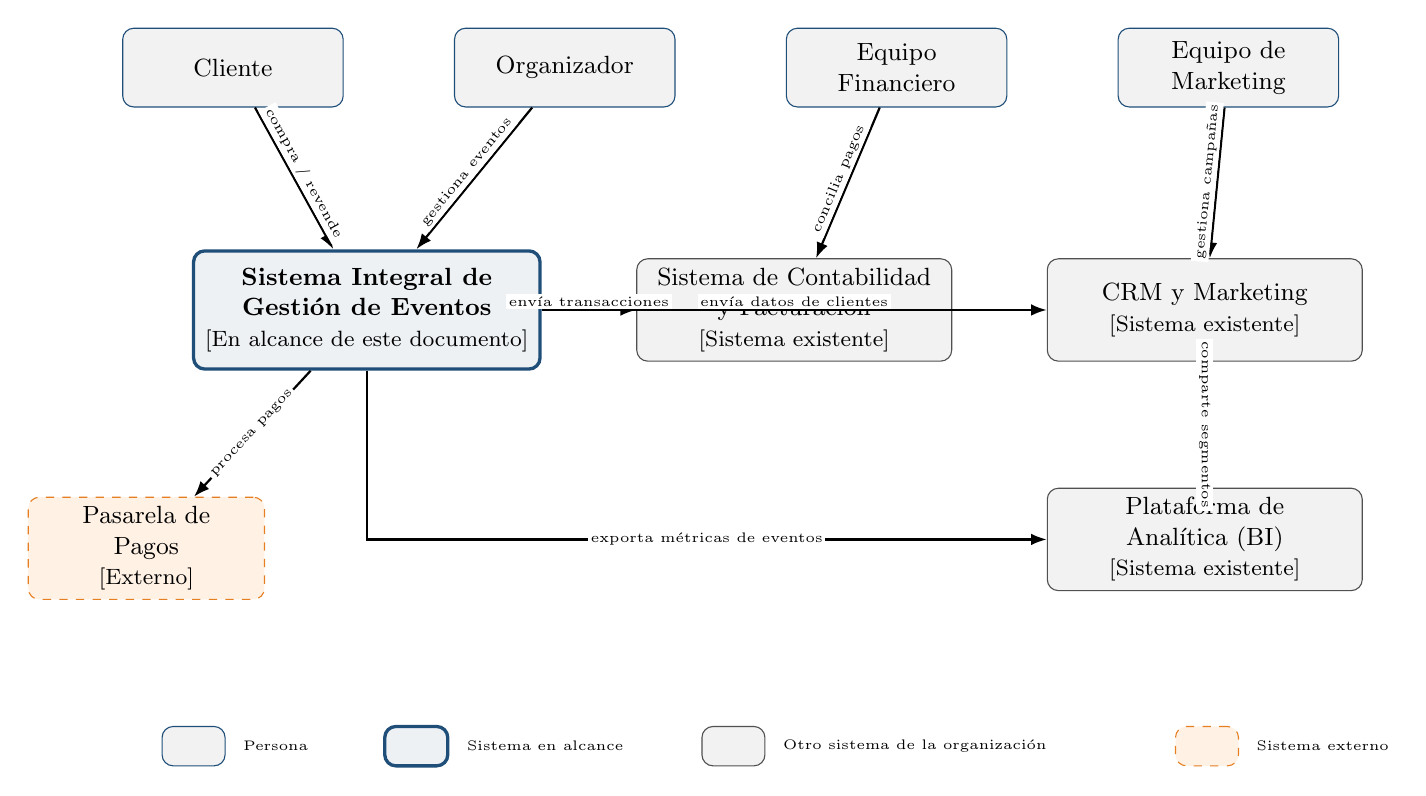
\begin{tikzpicture}[
persona/.style={draw=azul,rounded corners,fill=gris,minimum width=2.8cm,minimum height=1cm,align=center,font=\small},
sistemabox/.style={draw=azul,very thick,rounded corners,fill=azul!8,minimum width=4.4cm,minimum height=1.5cm,align=center,font=\small},
otrosistema/.style={draw=grisoscuro,rounded corners,fill=gris,minimum width=4cm,minimum height=1.3cm,align=center,font=\small},
ext/.style={draw=naranja,rounded corners,dashed,fill=orange!10,minimum width=3cm,minimum height=1cm,align=center,font=\small},
arr/.style={-{Latex[length=2mm]},thick},
lbl/.style={font=\tiny,fill=white,inner sep=1pt}
]
\node[persona] (cliente) {Cliente};
\node[persona,right=14mm of cliente] (organizador) {Organizador};
\node[persona,right=14mm of organizador] (finanzas) {Equipo\\Financiero};
\node[persona,right=14mm of finanzas] (marketing) {Equipo de\\Marketing};

\node[sistemabox,below=18mm of cliente,xshift=17mm] (sistema)
  {\textbf{Sistema Integral de}\\\textbf{Gestión de Eventos}\\\footnotesize [En alcance de este documento]};
\node[otrosistema,right=12mm of sistema] (contabilidad) {Sistema de Contabilidad\\y Facturación\\\footnotesize [Sistema existente]};
\node[otrosistema,right=12mm of contabilidad] (crm) {CRM y Marketing\\\footnotesize [Sistema existente]};

\node[otrosistema,below=16mm of crm] (bi) {Plataforma de\\Analítica (BI)\\\footnotesize [Sistema existente]};
\node[ext,below=16mm of sistema,xshift=-28mm] (pagos) {Pasarela de\\Pagos\\\footnotesize [Externo]};

\draw[arr] (cliente) -- (sistema) node[lbl,midway,sloped,above]{compra / revende};
\draw[arr] (organizador) -- (sistema) node[lbl,midway,sloped,above]{gestiona eventos};
\draw[arr] (finanzas) -- (contabilidad) node[lbl,midway,sloped,above]{concilia pagos};
\draw[arr] (marketing) -- (crm) node[lbl,midway,sloped,above]{gestiona campañas};

\draw[arr] (sistema) -- (contabilidad) node[lbl,midway,sloped,above]{envía transacciones};
\draw[arr] (sistema) -- (crm) node[lbl,midway,sloped,above]{envía datos de clientes};
\draw[arr] (sistema.south) |- (bi.west) node[lbl,pos=0.75,sloped]{exporta métricas de eventos};
\draw[arr] (crm) -- (bi) node[lbl,midway,sloped]{comparte segmentos};
\draw[arr] (sistema) -- (pagos) node[lbl,midway,sloped]{procesa pagos};

\node[persona,minimum width=8mm,minimum height=5mm,font=\tiny,below=16mm of pagos,xshift=6mm] (leg1) {};
\node[font=\tiny,right=1mm of leg1] {Persona};
\node[sistemabox,minimum width=8mm,minimum height=5mm,font=\tiny,right=20mm of leg1] (leg2) {};
\node[font=\tiny,right=1mm of leg2] {Sistema en alcance};
\node[otrosistema,minimum width=8mm,minimum height=5mm,font=\tiny,right=32mm of leg2] (leg3) {};
\node[font=\tiny,right=1mm of leg3] {Otro sistema de la organización};
\node[ext,minimum width=8mm,minimum height=5mm,font=\tiny,right=52mm of leg3] (leg4) {};
\node[font=\tiny,right=1mm of leg4] {Sistema externo};
\end{tikzpicture}
}
\caption{Diagrama de panorama de sistemas (\textit{System Landscape}, modelo C4).}
\end{figure}

\begin{longtable}{p{3.2cm}p{3.2cm}p{5.7cm}p{2.3cm}}
\toprule
\textbf{Origen} & \textbf{Destino} & \textbf{Descripción} & \textbf{Tecnología}\\
\midrule
Sistema Integral de Gestión de Eventos & Sistema de Contabilidad y Facturación & Envía las transacciones de venta, reventa, reembolsos y cobros de parqueadero para su registro contable. & HTTPS/REST (por lotes)\\
Sistema Integral de Gestión de Eventos & CRM y Marketing & Envía datos de clientes y su historial de compras para campañas y segmentación. & HTTPS/REST\\
Sistema Integral de Gestión de Eventos & Plataforma de Analítica (BI) & Exporta métricas de aforo, ventas y operación de eventos. & ETL / HTTPS\\
CRM y Marketing & Plataforma de Analítica (BI) & Comparte segmentos y campañas para el análisis conjunto con datos de eventos. & ETL\\
Sistema Integral de Gestión de Eventos & Pasarela de Pagos & Procesa compras, reventas y reembolsos. & HTTPS/REST\\
\bottomrule
\caption{Relaciones del diagrama de panorama de sistemas.}
\end{longtable}

\section{Diagrama dinámico (Dynamic Diagram) --- Reventa de una entrada}

\textbf{Tipo:} diagrama dinámico (\textit{Dynamic Diagram}). \textbf{Alcance:} muestra, con
interacciones numeradas al estilo de un diagrama de secuencia, cómo colaboran los contenedores del
Nivel 2 para resolver el caso de uso complejo \textbf{CU-006 --- Gestión del Mercado Secundario de
Entradas} cuando un comprador adquiere una entrada publicada en reventa. \textbf{Audiencia:}
arquitectos y desarrolladores.

\begin{figure}[H]
\centering
\resizebox{\textwidth}{!}{
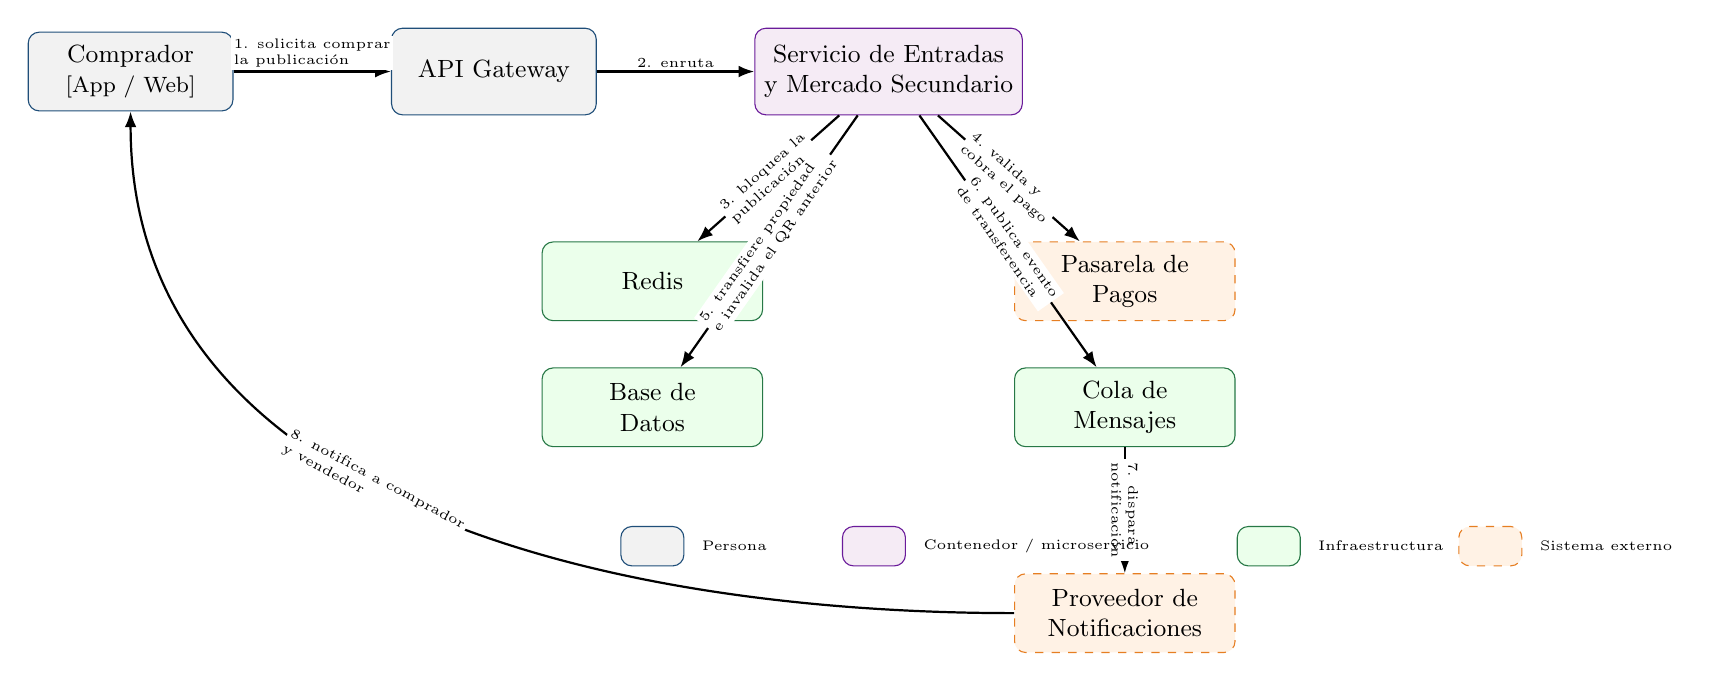
\begin{tikzpicture}[
persona/.style={draw=azul,rounded corners,fill=gris,minimum width=2.6cm,minimum height=1cm,align=center,font=\small},
contenedor/.style={draw=azul,rounded corners,fill=gris,minimum width=2.6cm,minimum height=1.1cm,align=center,font=\small},
microservicio/.style={draw=morado,rounded corners,fill=violet!8,minimum width=2.9cm,minimum height=1.1cm,align=center,font=\small},
infra/.style={draw=verde,rounded corners,fill=green!8,minimum width=2.8cm,minimum height=1cm,align=center,font=\small},
ext/.style={draw=naranja,rounded corners,dashed,fill=orange!10,minimum width=2.8cm,minimum height=1cm,align=center,font=\small},
arr/.style={-{Latex[length=2mm]},thick},
lbl/.style={font=\tiny,fill=white,inner sep=1pt,align=left}
]
\node[persona] (comprador) {Comprador\\\footnotesize [App / Web]};
\node[contenedor,right=20mm of comprador] (gw) {API Gateway};
\node[microservicio,right=20mm of gw] (ms) {Servicio de Entradas\\y Mercado Secundario};
\node[infra,below=16mm of ms,xshift=-30mm] (redis) {Redis};
\node[ext,below=16mm of ms,xshift=30mm] (pasarela) {Pasarela de\\Pagos};
\node[infra,below=32mm of ms,xshift=-30mm] (bd) {Base de\\Datos};
\node[infra,below=32mm of ms,xshift=30mm] (cola) {Cola de\\Mensajes};
\node[ext,below=16mm of cola] (notif) {Proveedor de\\Notificaciones};

\draw[arr] (comprador) -- (gw) node[lbl,midway,sloped,above]{1. solicita comprar\\la publicación};
\draw[arr] (gw) -- (ms) node[lbl,midway,sloped,above]{2. enruta};
\draw[arr] (ms) -- (redis) node[lbl,midway,sloped]{3. bloquea la\\publicación};
\draw[arr] (ms) -- (pasarela) node[lbl,midway,sloped]{4. valida y\\cobra el pago};
\draw[arr] (ms) -- (bd) node[lbl,midway,sloped]{5. transfiere propiedad\\e invalida el QR anterior};
\draw[arr] (ms) -- (cola) node[lbl,midway,sloped]{6. publica evento\\de transferencia};
\draw[arr] (cola) -- (notif) node[lbl,midway,sloped]{7. dispara\\notificación};
\draw[arr] (notif.west) to[out=180,in=-90] node[lbl,pos=0.55,sloped]{8. notifica a comprador\\y vendedor} (comprador.south);

\node[persona,minimum width=8mm,minimum height=5mm,font=\tiny,below=10mm of bd] (leg1) {};
\node[font=\tiny,right=1mm of leg1] {Persona};
\node[microservicio,minimum width=8mm,minimum height=5mm,font=\tiny,right=20mm of leg1] (leg2) {};
\node[font=\tiny,right=1mm of leg2] {Contenedor / microservicio};
\node[infra,minimum width=8mm,minimum height=5mm,font=\tiny,right=42mm of leg2] (leg3) {};
\node[font=\tiny,right=1mm of leg3] {Infraestructura};
\node[ext,minimum width=8mm,minimum height=5mm,font=\tiny,right=20mm of leg3] (leg4) {};
\node[font=\tiny,right=1mm of leg4] {Sistema externo};
\end{tikzpicture}
}
\caption{Diagrama dinámico --- reventa de una entrada (CU-006, modelo C4). Los números en cada
flecha indican el orden de la interacción.}
\end{figure}

\begin{longtable}{p{1cm}p{4cm}p{7.4cm}}
\toprule
\textbf{Paso} & \textbf{Interacción} & \textbf{Descripción}\\
\midrule
1 & Comprador $\rightarrow$ API Gateway & El comprador confirma la compra de una entrada publicada en el mercado secundario.\\
2 & API Gateway $\rightarrow$ Servicio de Entradas & Enruta la solicitud autenticada hacia el microservicio responsable.\\
3 & Servicio de Entradas $\rightarrow$ Redis & Bloquea temporalmente la publicación para impedir que otro comprador la adquiera simultáneamente.\\
4 & Servicio de Entradas $\rightarrow$ Pasarela de Pagos & Valida el medio de pago y cobra el valor de la entrada.\\
5 & Servicio de Entradas $\rightarrow$ Base de Datos & Transfiere la propiedad de la entrada e invalida el código QR anterior.\\
6 & Servicio de Entradas $\rightarrow$ Cola de Mensajes & Publica el evento \texttt{ENTRADA\_TRANSFERIDA} para su procesamiento asíncrono.\\
7 & Cola de Mensajes $\rightarrow$ Proveedor de Notificaciones & Dispara el envío de notificaciones desacoplado del flujo principal.\\
8 & Proveedor de Notificaciones $\rightarrow$ Comprador / Vendedor & Notifica la confirmación de la transferencia y el nuevo código QR.\\
\bottomrule
\caption{Secuencia de interacciones del diagrama dinámico.}
\end{longtable}

\section{Diagrama de despliegue (Deployment Diagram)}

\textbf{Tipo:} diagrama de despliegue (\textit{Deployment Diagram}). \textbf{Alcance:} muestra en
qué nodos de infraestructura real se despliegan los contenedores del Nivel 2: dispositivos del
usuario, red de distribución de contenido, clúster de aplicación y clústeres de datos/mensajería,
en un ambiente de producción en la nube. \textbf{Audiencia:} arquitectos, DevOps e infraestructura.

\begin{figure}[H]
\centering
\resizebox{\textwidth}{!}{
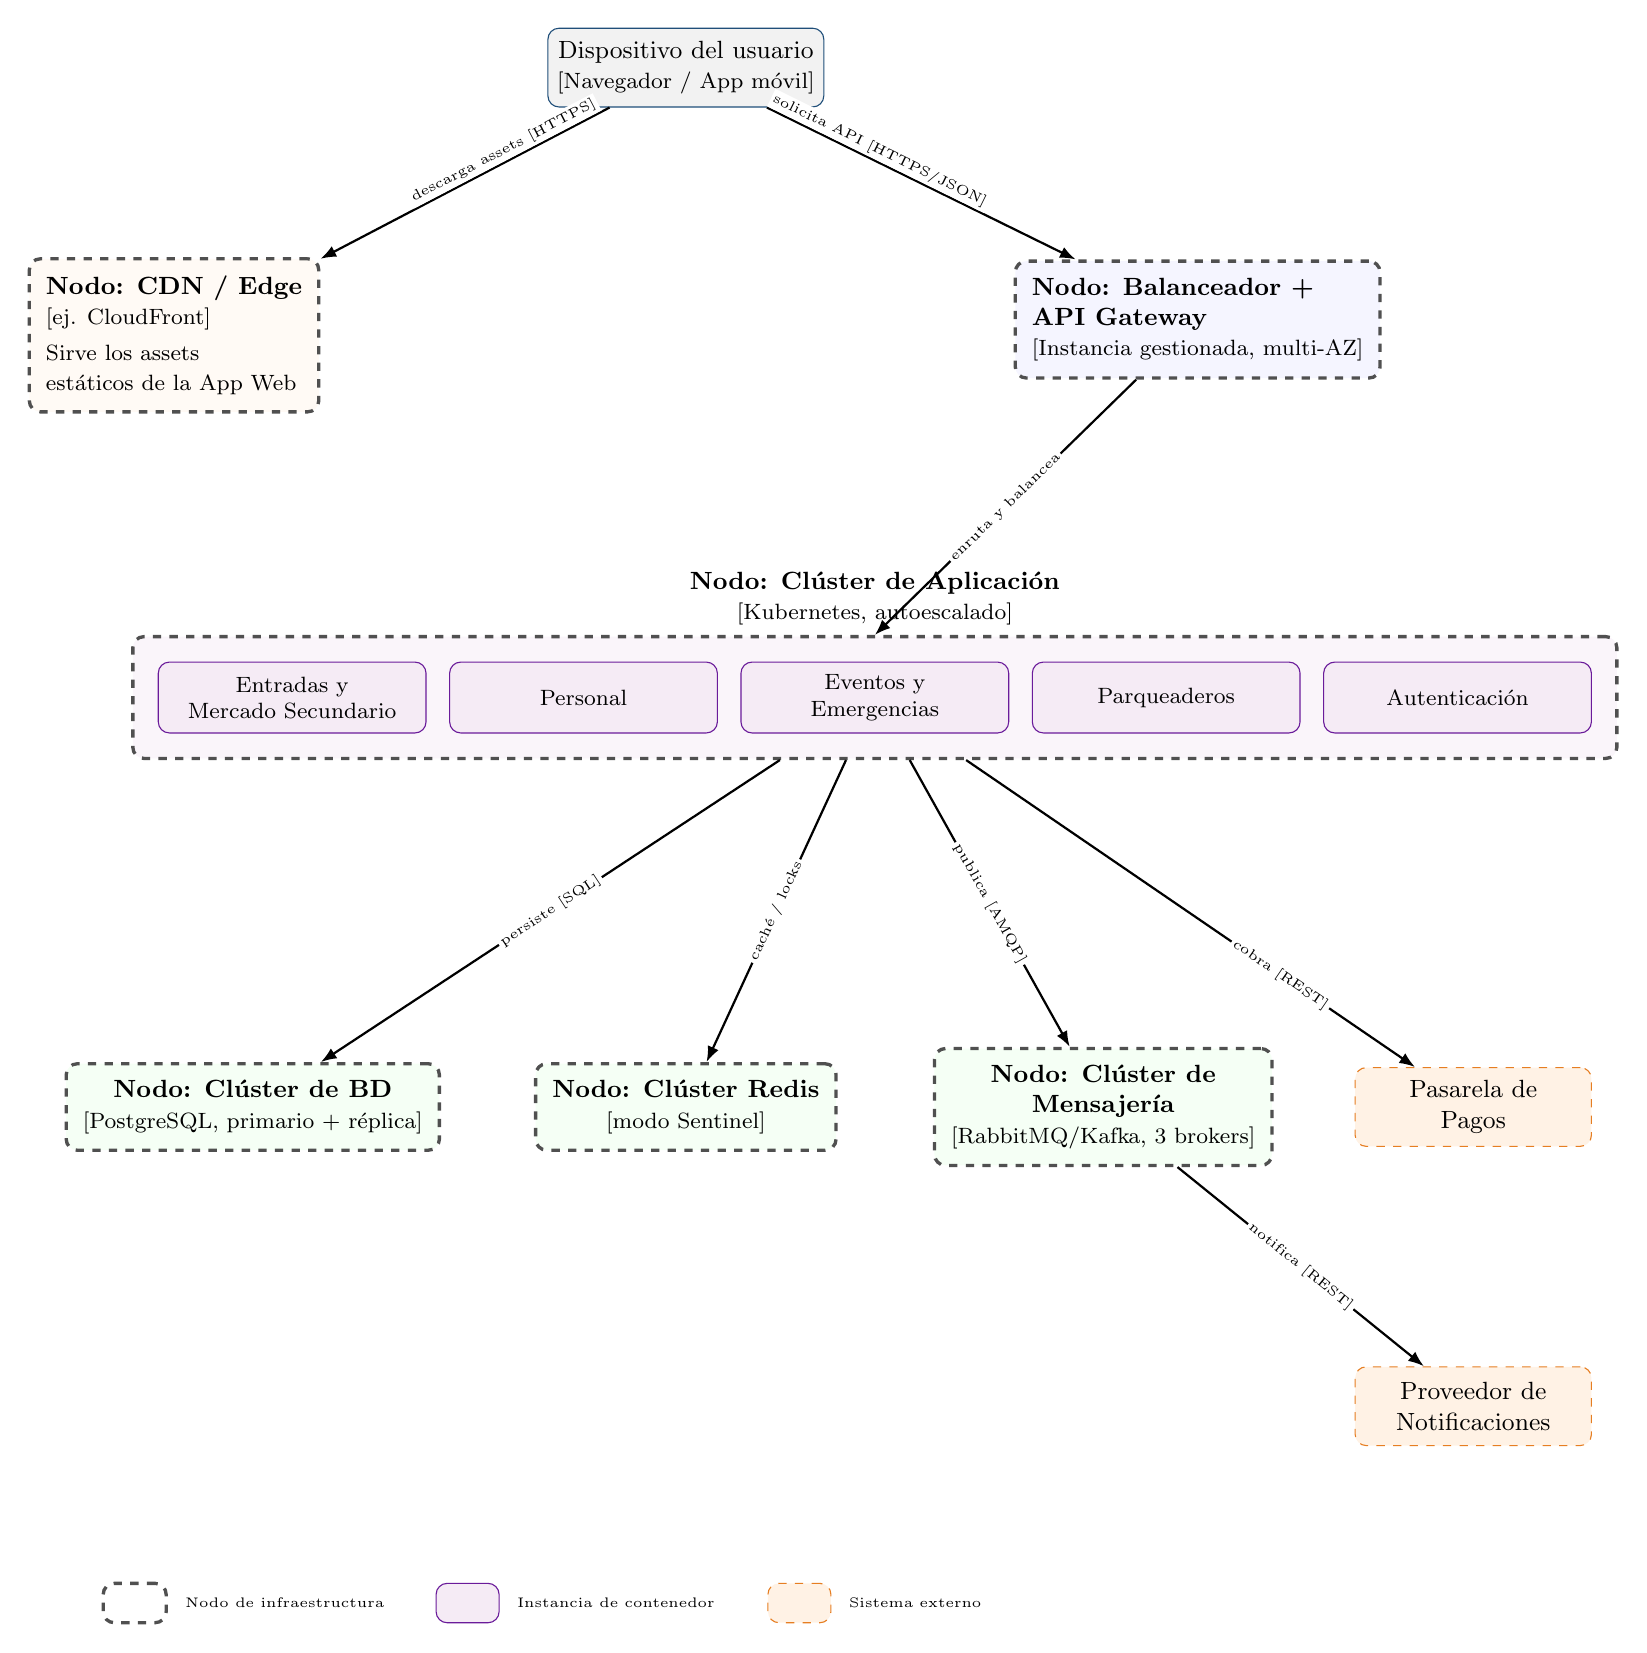
\begin{tikzpicture}[
nodo/.style={draw=grisoscuro,very thick,dashed,rounded corners,align=center,font=\small,inner sep=6pt},
persona/.style={draw=azul,rounded corners,fill=gris,minimum width=2.8cm,minimum height=1cm,align=center,font=\small},
contenedor/.style={draw=azul,rounded corners,fill=gris,minimum width=3.4cm,minimum height=0.9cm,align=center,font=\footnotesize},
microservicio/.style={draw=morado,rounded corners,fill=violet!8,minimum width=3.4cm,minimum height=0.9cm,align=center,font=\footnotesize},
infra/.style={draw=verde,rounded corners,fill=green!8,minimum width=3.4cm,minimum height=0.9cm,align=center,font=\footnotesize},
ext/.style={draw=naranja,rounded corners,dashed,fill=orange!10,minimum width=3cm,minimum height=1cm,align=center,font=\small},
arr/.style={-{Latex[length=2mm]},thick},
lbl/.style={font=\tiny,fill=white,inner sep=1pt}
]
\node[persona] (usuario) at (7,0) {Dispositivo del usuario\\\footnotesize [Navegador / App móvil]};

\node[nodo,fill=orange!4,align=left] (cdn) at (0.5,-3.4)
  {\textbf{Nodo: CDN / Edge}\\\footnotesize [ej. CloudFront]\\[2pt]\footnotesize Sirve los assets\\\footnotesize estáticos de la App Web};
\node[nodo,fill=blue!4,align=left] (edge) at (13.5,-3.2)
  {\textbf{Nodo: Balanceador +}\\\textbf{API Gateway}\\\footnotesize [Instancia gestionada, multi-AZ]};

\node[microservicio] (p1) at (2,-8) {Entradas y\\Mercado Secundario};
\node[microservicio] (p2) at (5.7,-8) {Personal};
\node[microservicio] (p3) at (9.4,-8) {Eventos y\\Emergencias};
\node[microservicio] (p4) at (13.1,-8) {Parqueaderos};
\node[microservicio] (p5) at (16.8,-8) {Autenticación};
\begin{scope}[on background layer]
\node[nodo,fill=violet!4,fit=(p1)(p2)(p3)(p4)(p5),inner sep=9pt,
  label={[font=\small\bfseries,align=center]above:Nodo: Clúster de Aplicación\\\footnotesize\normalfont[Kubernetes, autoescalado]}] (k8s) {};
\end{scope}

\node[nodo,fill=green!4] (bdnodo) at (1.5,-13.2) {\textbf{Nodo: Clúster de BD}\\\footnotesize [PostgreSQL, primario + réplica]};
\node[nodo,fill=green!4] (redisnodo) at (7,-13.2) {\textbf{Nodo: Clúster Redis}\\\footnotesize [modo Sentinel]};
\node[nodo,fill=green!4] (colanodo) at (12.3,-13.2) {\textbf{Nodo: Clúster de}\\\textbf{Mensajería}\\\footnotesize [RabbitMQ/Kafka, 3 brokers]};
\node[ext] (pagos) at (17,-13.2) {Pasarela de\\Pagos};

\node[ext] (notif) at (17,-17) {Proveedor de\\Notificaciones};

\draw[arr] (usuario) -- (cdn) node[lbl,pos=0.35,sloped,above]{descarga assets [HTTPS]};
\draw[arr] (usuario) -- (edge) node[lbl,pos=0.35,sloped,above]{solicita API [HTTPS/JSON]};
\draw[arr] (edge) -- (k8s.north) node[lbl,midway,sloped]{enruta y balancea};
\draw[arr] (k8s) -- (bdnodo) node[lbl,midway,sloped]{persiste [SQL]};
\draw[arr] (k8s) -- (redisnodo) node[lbl,midway,sloped]{caché / locks};
\draw[arr] (k8s) -- (colanodo) node[lbl,midway,sloped]{publica [AMQP]};
\draw[arr] (k8s) -- (pagos) node[lbl,pos=0.7,sloped]{cobra [REST]};
\draw[arr] (colanodo) -- (notif) node[lbl,midway,sloped]{notifica [REST]};

\node[nodo,minimum width=8mm,minimum height=5mm,font=\tiny,inner sep=1pt] (leg1) at (0,-19.5) {};
\node[font=\tiny,right=1mm of leg1] {Nodo de infraestructura};
\node[microservicio,minimum width=8mm,minimum height=5mm,font=\tiny,right=34mm of leg1] (leg2) {};
\node[font=\tiny,right=1mm of leg2] {Instancia de contenedor};
\node[ext,minimum width=8mm,minimum height=5mm,font=\tiny,right=34mm of leg2] (leg3) {};
\node[font=\tiny,right=1mm of leg3] {Sistema externo};
\end{tikzpicture}
}
\caption{Diagrama de despliegue (\textit{Deployment}, modelo C4).}
\end{figure}

\begin{longtable}{p{3.6cm}p{3.6cm}p{5.2cm}p{2cm}}
\toprule
\textbf{Nodo origen} & \textbf{Nodo destino} & \textbf{Descripción} & \textbf{Tecnología}\\
\midrule
Dispositivo del usuario & CDN / Edge & Descarga los archivos estáticos de la aplicación web. & HTTPS\\
Dispositivo del usuario & Balanceador + API Gateway & Envía las solicitudes de la API. & HTTPS/JSON\\
Balanceador + API Gateway & Clúster de Aplicación & Enruta y balancea la carga entre las réplicas de cada microservicio. & HTTPS/JSON\\
Clúster de Aplicación & Clúster de BD & Persiste y consulta los datos de cada dominio. & SQL\\
Clúster de Aplicación & Clúster Redis & Caché de lectura y bloqueos temporales de concurrencia. & Redis\\
Clúster de Aplicación & Clúster de Mensajería & Publica eventos de dominio para procesamiento asíncrono. & AMQP\\
Clúster de Aplicación & Pasarela de Pagos & Procesa cobros y reembolsos. & HTTPS/REST\\
Clúster de Mensajería & Proveedor de Notificaciones & Dispara notificaciones push, correo y SMS. & HTTPS/REST\\
\bottomrule
\caption{Relaciones del diagrama de despliegue.}
\end{longtable}

\section{Verificación contra el checklist oficial de C4}

Los seis diagramas (Contexto, Contenedores, Componentes, Panorama de Sistemas, Dinámico y
Despliegue) se validaron contra el \textit{Software architecture diagram review checklist} oficial
de \href{https://c4model.com/diagrams/checklist}{c4model.com/diagrams/checklist}. La tabla
reproduce cada criterio del checklist oficial y cómo lo satisface este documento.

\begin{longtable}{p{9.5cm}p{4.5cm}}
\toprule
\textbf{Criterio (General)} & \textbf{Cumple}\\
\midrule
¿El diagrama tiene título? & Sí, en el encabezado de cada sección y en cada \textit{caption}.\\
¿Se entiende el tipo de diagrama? & Sí, indicado explícitamente como \textbf{Tipo:} al inicio de cada sección.\\
¿Se entiende el alcance del diagrama? & Sí, indicado explícitamente como \textbf{Alcance:} al inicio de cada sección.\\
¿El diagrama tiene leyenda/clave? & Sí, todos incluyen leyenda de formas y colores.\\
\midrule
\textbf{Criterio (Elementos)} & \textbf{Cumple}\\
\midrule
¿Cada elemento tiene nombre? & Sí.\\
¿Se entiende el tipo de cada elemento (persona, sistema, contenedor, componente, nodo)? & Sí (ver leyenda de cada figura).\\
¿Se entiende qué hace cada elemento? & Sí, cada nodo incluye una descripción o etiqueta de tecnología entre corchetes.\\
¿Se entienden las tecnologías asociadas a cada elemento? & Sí (anotadas entre corchetes en cada nodo).\\
¿Se entienden todas las siglas y abreviaturas? & Sí: SPA, API, AMQP, ETL, BI, CRM, CDN, multi-AZ se explicitan la primera vez que aparecen.\\
¿Se entiende el significado de los colores usados? & Sí (ver leyenda): azul = aplicación/contenedor propio, morado = microservicio/componente, verde = infraestructura, naranja punteado = sistema/servicio externo, gris = persona u otro sistema de la organización.\\
¿Se entiende el significado de las formas usadas? & Sí: una sola forma (rectángulo de esquinas redondeadas) en todo el documento; solo cambia el color/borde según el tipo de elemento.\\
¿Se entiende el significado de los íconos usados? & No aplica: este documento no usa íconos, solo color y texto.\\
¿Se entiende el significado de los bordes punteados? & Sí: punteado = sistema externo, referencia a un elemento de otro nivel, o nodo de infraestructura física (ver leyenda de cada figura).\\
¿Se entiende el significado del tamaño de los elementos? & Sí: el tamaño es uniforme dentro de cada tipo de elemento y no codifica información adicional (se aclara para evitar ambigüedad).\\
\midrule
\textbf{Criterio (Relaciones)} & \textbf{Cumple}\\
\midrule
¿Cada flecha tiene una etiqueta que describe la relación? & Sí.\\
¿La descripción coincide con la dirección de la flecha? & Sí.\\
¿Se entienden las tecnologías/protocolos de cada relación? & Sí (ver tablas de relaciones al pie de cada figura).\\
¿Se entienden todas las siglas y abreviaturas de las relaciones? & Sí (HTTPS, REST, SQL, AMQP, ETL se usan de forma consistente).\\
¿Se entiende el significado de los colores usados en las relaciones? & Sí: todas las flechas usan el mismo color y estilo; no se codifica información adicional por color.\\
¿Se entiende el significado de las cabezas de flecha? & Sí: una sola convención (flecha simple) en todo el documento, siempre en el sentido \textit{origen} $\rightarrow$ \textit{destino}.\\
¿Se entiende el significado del estilo de línea (sólida/punteada)? & Sí: línea sólida en todas las relaciones; no se usa línea punteada para relaciones (solo para bordes de elementos externos/nodos).\\
\bottomrule
\caption{Verificación contra el checklist de c4model.com.}
\end{longtable}

\section{Conclusión}

Los seis diagramas de este documento cubren el modelo C4 completo, salvo el Nivel 4 (Código), que
se excluye deliberadamente por las razones explicadas en la introducción. Los tres niveles
jerárquicos documentan de forma progresiva la arquitectura del Sistema Integral de Gestión de
Eventos: desde su relación con los usuarios y sistemas externos (Nivel 1: Contexto), pasando por
sus aplicaciones, microservicios e infraestructura de soporte (Nivel 2: Contenedores), hasta el
detalle interno del componente más complejo del sistema, el Servicio de Entradas y Mercado
Secundario (Nivel 3: Componentes, CU-006). Los tres diagramas auxiliares complementan esa vista
jerárquica: el \textbf{Panorama de Sistemas} ubica al sistema dentro del ecosistema de software de
la organización (contabilidad, CRM y analítica); el \textbf{Dinámico} muestra, paso a paso, cómo
colaboran los contenedores para resolver la reventa de una entrada; y el \textbf{Despliegue}
aterriza los contenedores en nodos de infraestructura real (CDN, balanceador, clúster de
aplicación, clústeres de datos y mensajería). Cada uno de los seis diagramas fue verificado contra
el checklist oficial de c4model.com, garantizando que título, alcance, leyenda, tipos de elemento y
tecnologías de cada relación queden explícitos. Este documento debe leerse en conjunto con
\textit{Atributos de Calidad y Propuesta Arquitectónica}, que sustenta las decisiones que aquí se
representan gráficamente.

\end{document}
